\section{Experimento 2: Red hogareña}

\subsection{Descripción del contexto}

El experimento fue realizado en una red doméstica, por medio de una conexión Wi-Fi de Fibertel. Al momento de tomar las mediciones estaban conectados a la red una laptop, una smart TV, un celular y una tablet, entre otras cosas. La fecha de la captura fue Sábado 7 de Octubre de 2017.

\subsection{Descripción de la captura}

%% distribucion de protocolos (grafico)
Capturamos 10000 paquetes. A continuación se muestra la distribución de protocolos dentro de la captura.
\begin{figure}[H]
\centering
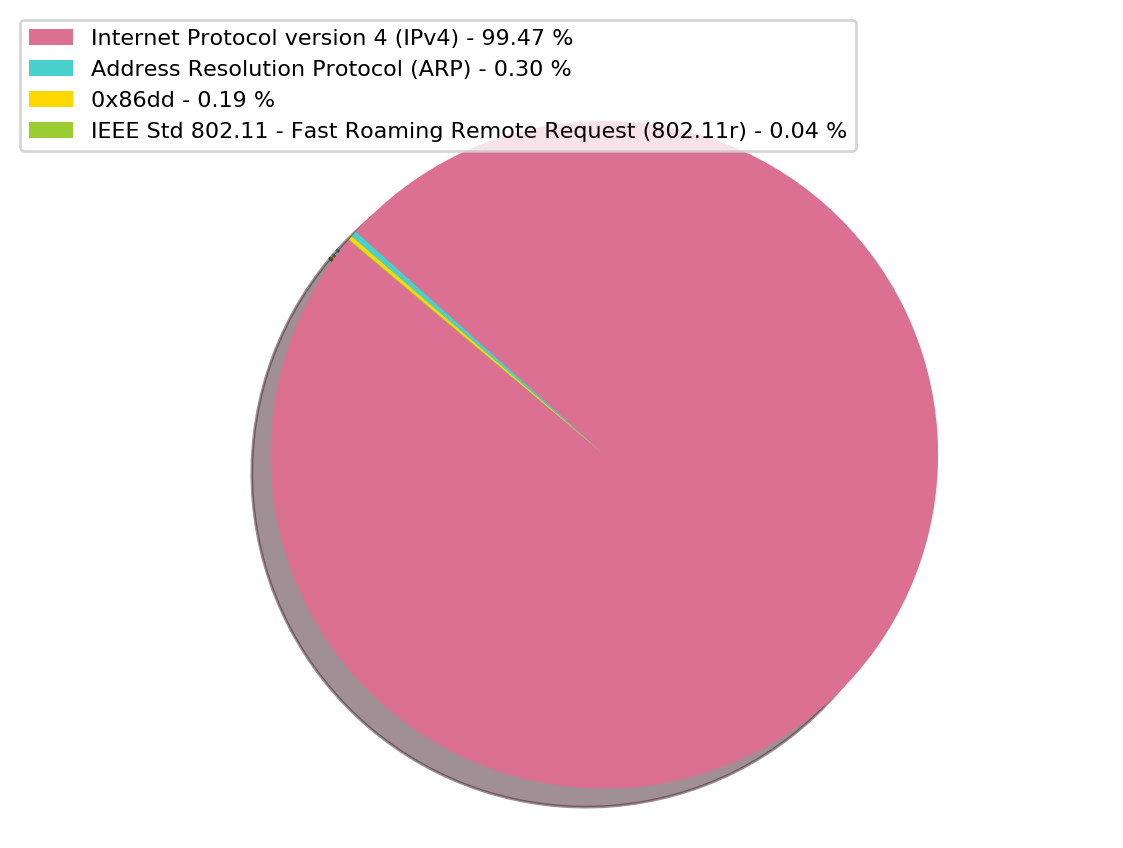
\includegraphics[width=0.7\textwidth]{protocolosRed2.png}
\caption{Gráfico que muestra la distribución de protocolos en la red.}
\label{protocolos2}
\end{figure}

Observamos 4 tipos de paquetes distintos, la mayoría de los cuales son de tipo IPv4. Además, hay BLA\% de paquetes ARP.
%% grafico de broadcast
\begin{figure}[H]
\centering
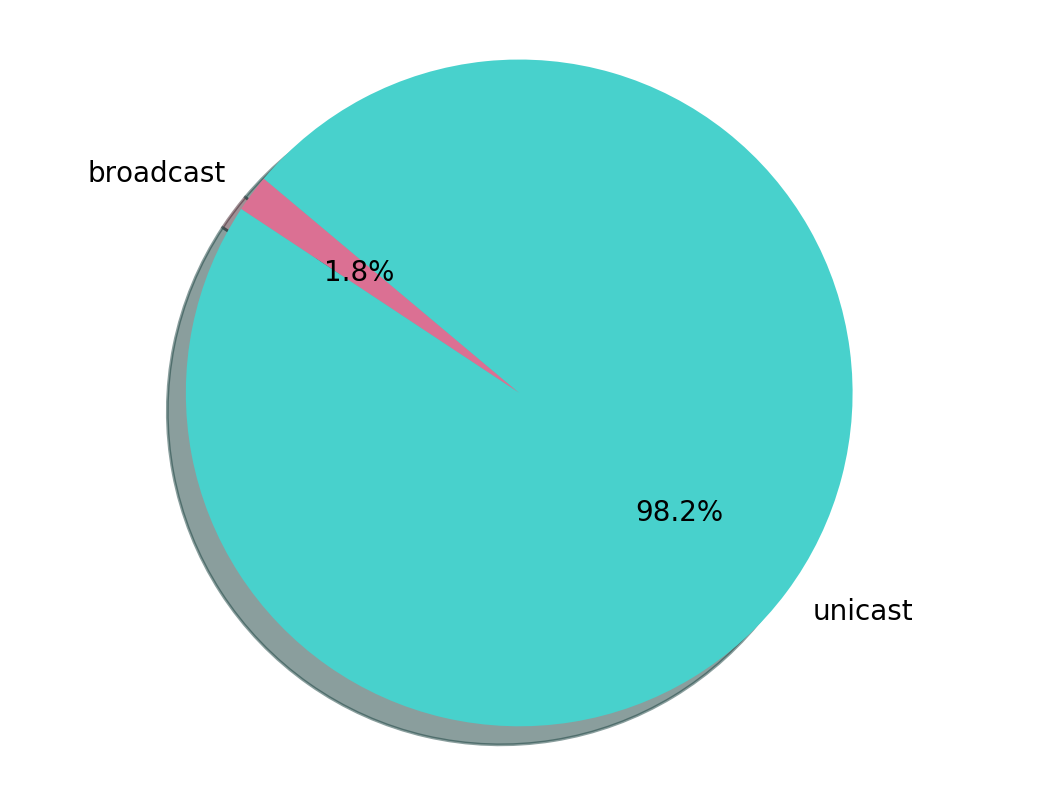
\includegraphics[width=0.7\textwidth]{broadcastRed2.png}
\caption{Gráfico que muestra los porcentajes de tráfico broadcast y unicast.}
\label{broadcast2}
\end{figure}

\subsection{Análisis de la captura}

%% grafico entropia S1
\begin{figure}[H]
\centering
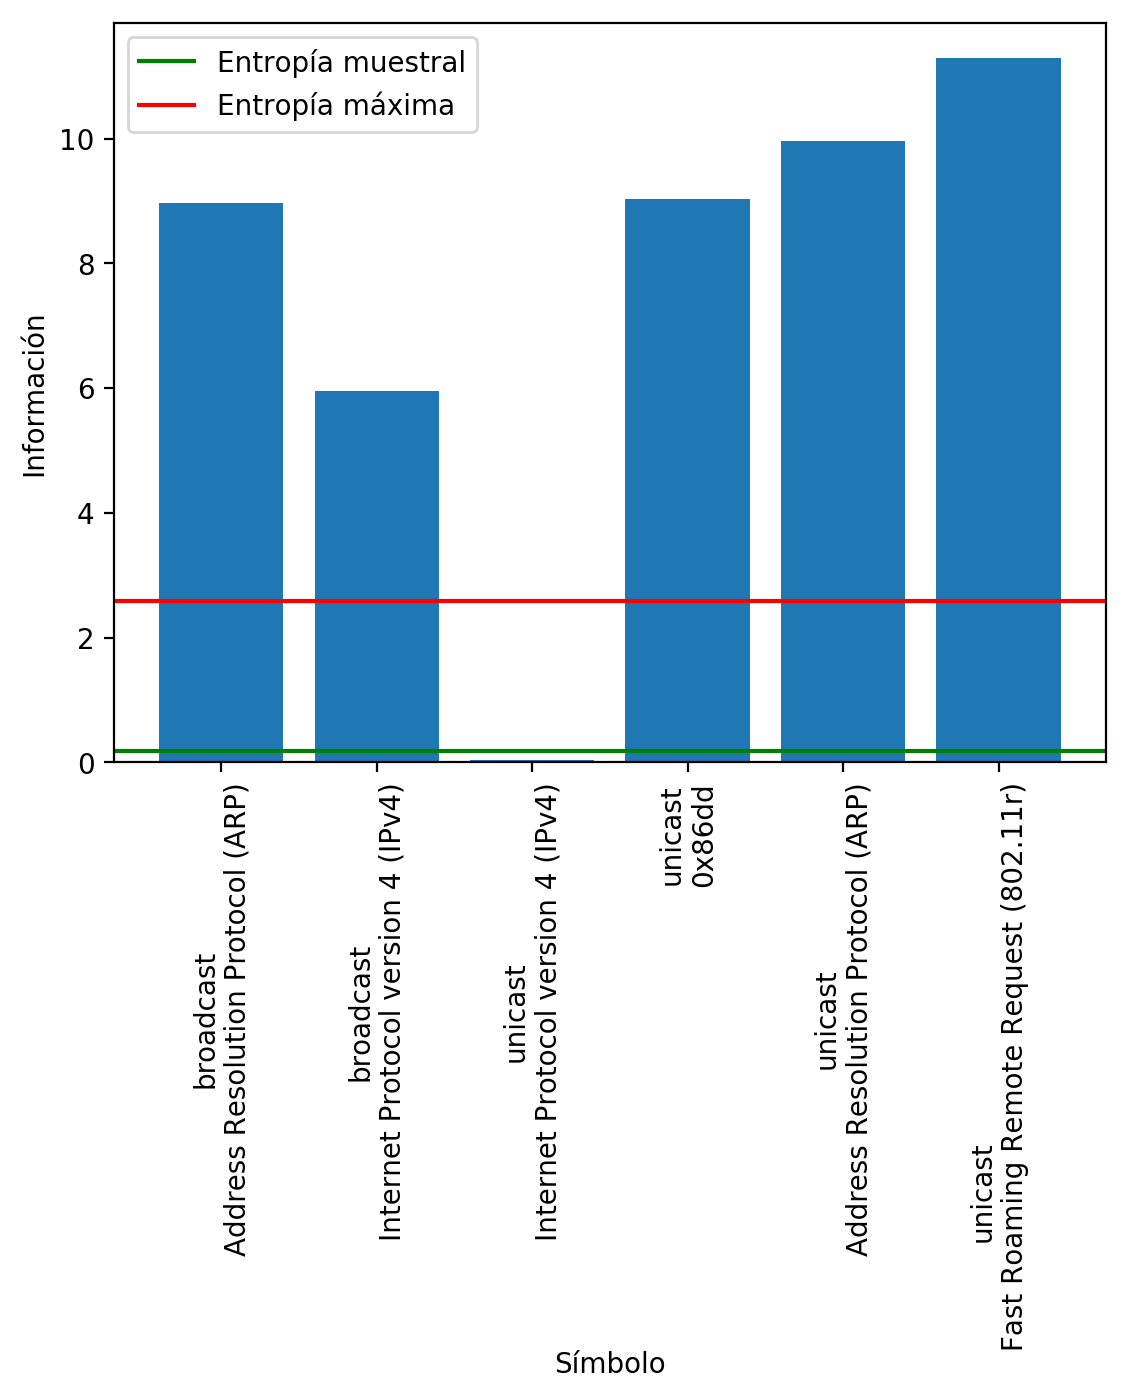
\includegraphics[width=0.7\textwidth]{entropiaS1Red2.png}
\caption{Gráfico de la información de los símbolos de la fuente $S_1$ observados en esta red. Se muestra la entropía muestral de $S_1$ y su entropía máxima.}
\label{entropias1_2}
\end{figure}

%% grafico entropia S2
\begin{figure}[H]
\centering
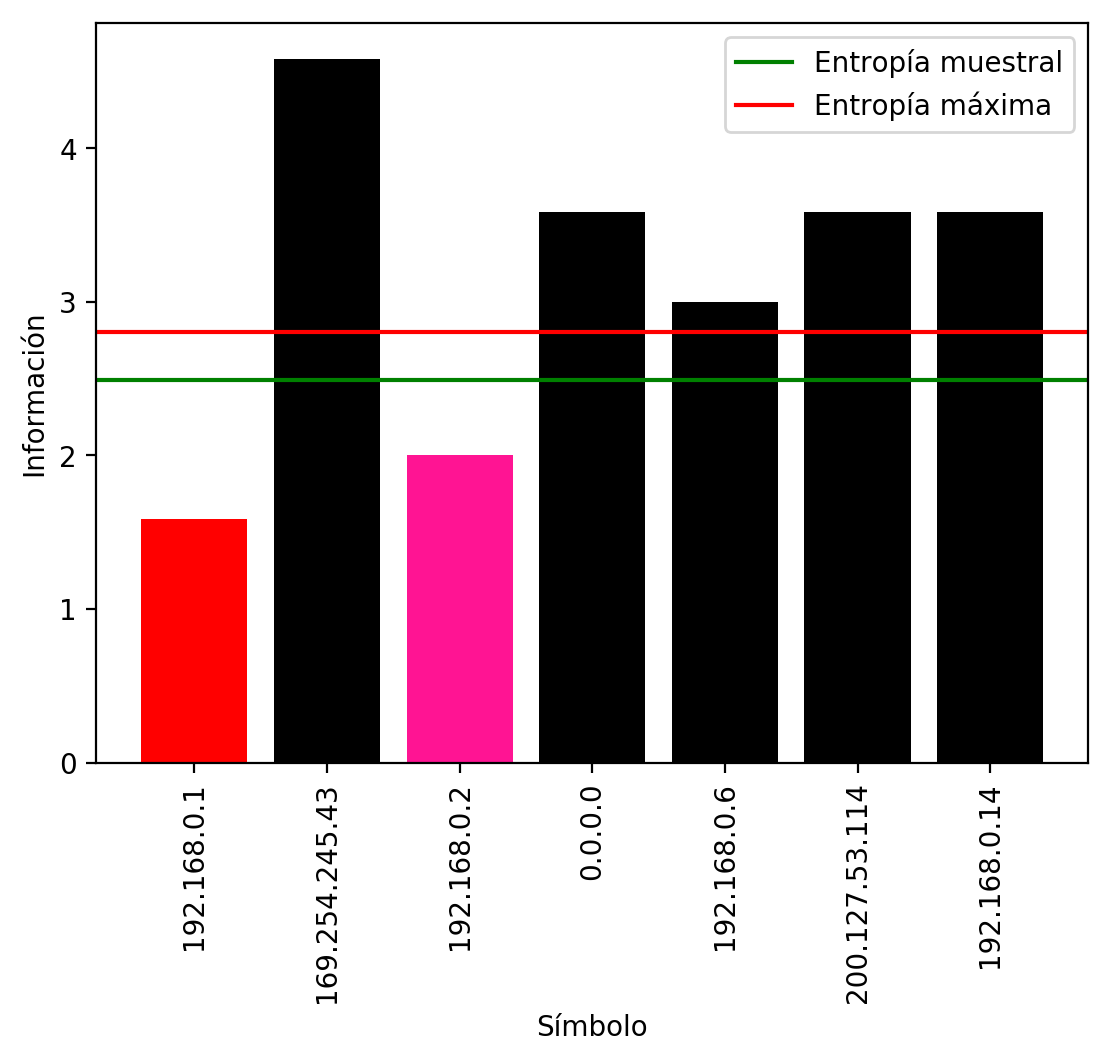
\includegraphics[width=0.7\textwidth]{entropiaS2Red2.png}
\caption{Gráfico de la información de los símbolos de la fuente $S_2$ observados en esta red. Se muestra la entropía muestral de $S_2$ y su entropía máxima.}
\label{entropias2_2}
\end{figure}

%% red ARP
\begin{figure}[H]
\centering
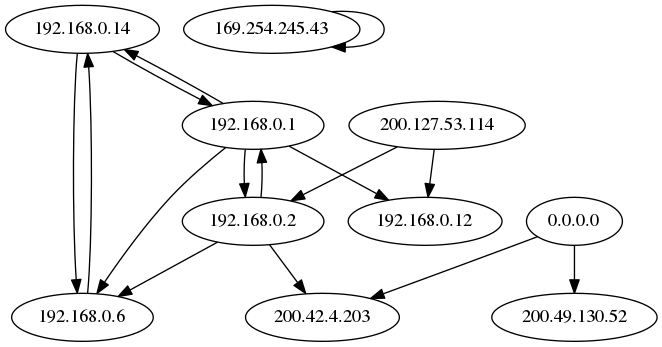
\includegraphics[width=0.7\textwidth]{grafoRed2.png}
\caption{Grafo de la red de mensajes ARP subyacente.}
\label{grafo2}
\end{figure}
